\chapter{Métodos e Desenvolvimento}
\label{cap:desen}
Este capítulo descreve as etapas de desenvolvimento e as metodologias empregadas neste trabalho. Buscaram-se estratégias sem intrusão ou grandes modificações nas políticas de escalonamento já implementadas pelo \textit{framework}. Nas Seções \ref{sec:collector} e \ref{sec:zookeeper} são apresentados em maior detalhe os coletores de contexto e a ferramenta de comunicação distribuída utilizados neste trabalho, respectivamente. Finalmente, na Seção \ref{sec:solucao} explica-se em profundidade a solução implementada neste trabalho.

%-------------------------------------------------------------------
\section{Coletores de Contexto}
\label{sec:collector}

%TODO descrição geral.
%TODO diagrama de classes

Após um estudo aprofundado dos escalonadores do Hadoop, ficou claro que o Capacity Scheduler já está estruturado de maneira a oferecer escalabilidade e um desempenho satisfatório. Porém, este escalonador possui um ponto fraco, o qual é exposto quando utilizado em um ambiente compartilhado, ele só recebe informações sobre os Node Managers no momento da inicialização destes, e ainda, a informação é obtida de um arquivo estático de configuração. Sabendo que o escalonamento é fortemente ligado com a disponibilidade de recursos e, portanto, uma informação errada pode prejudicar o desempenho do algoritmo, é importante que a informação sobre os Node Managers sempre esteja atualizada. Com base nestas observações, o primeiro passo para a solução é a coleta de dados dos Node managers.

Em um primeiro momento, buscou-se diminuir a dependência nos arquivos XML para a configuração dos recursos dos Node Managers com intuito de facilitar a configuração inicial dos nós e futuramente utilizar este mesmo mecanismo para a inclusão do suporte ao compartilhamento dos recursos. Para isto, fez-se necessário o desenvolvimento de um conjunto de coletores de contexto capazes de coletar de maneira eficiente os recursos da máquina em questão no momento da inicialização do serviço Node Manager e posteriormente, no momento do registro no Resource Manager fornecer a informação correta.

Embora esta adição já facilite a utilização do Hadoop em um \textit{cluster} de natureza heterogênea ou dinâmica, ainda não é suficiente para que o Hadoop seja utilizado eficientemente em um \textit{cluster} compartilhado. A razão para esta afirmação é que, embora a informação esteja correta no momento de inicialização, é possível que durante a execução das aplicações de \textit{MapReduce} os recursos comecem a ser utilizados por outros usuários, diminuindo a capacidade disponível para o Hadoop.

Com objetivo de solucionar o problema causado pelo compartilhamento, é necessário que a coleta de dados ocorra não apenas na inicialização do Node Manager mas ao longo da execução do serviço em intervalos periódicos.

O coletor escolhido para a tarefa foi o coletor desenvolvido pelo projeto PER-MARE \cite{Collector}, o qual utiliza a interface padrão do Java para monitoramento, OperatingSystemMXBean \cite{MXBean}.

A implementação deste coletor de contexto é baseada em uma interface, uma classe abstrata e as classes de coleta dos recursos desejados. Devido ao seu projeto, coletores de novas informações podem ser facilmente criados, aumentando assim a quantidade de informação disponível para o escalonador.

A interface OperatingSystemMXBean, possibilita o acesso às informações do sistema no qual a JVM está sendo executada. Uma vez que a classe abstrata implementa esta interface, todas suas herdeiras terão acesso à ela.

As classes utilizadas neste trabalho fazem a coleta de memória física disponível e processadores disponíveis, os recursos suportados por padrão no Hadoop. É possível visualizar o digrama de classes na figura \ref{fig:collectorUML}, onde estão presentes alguns exemplos de possíveis coletores a serem utilizados.

%TODO fazer outro DC
\begin{figure}[!hbtn]
   \centering
   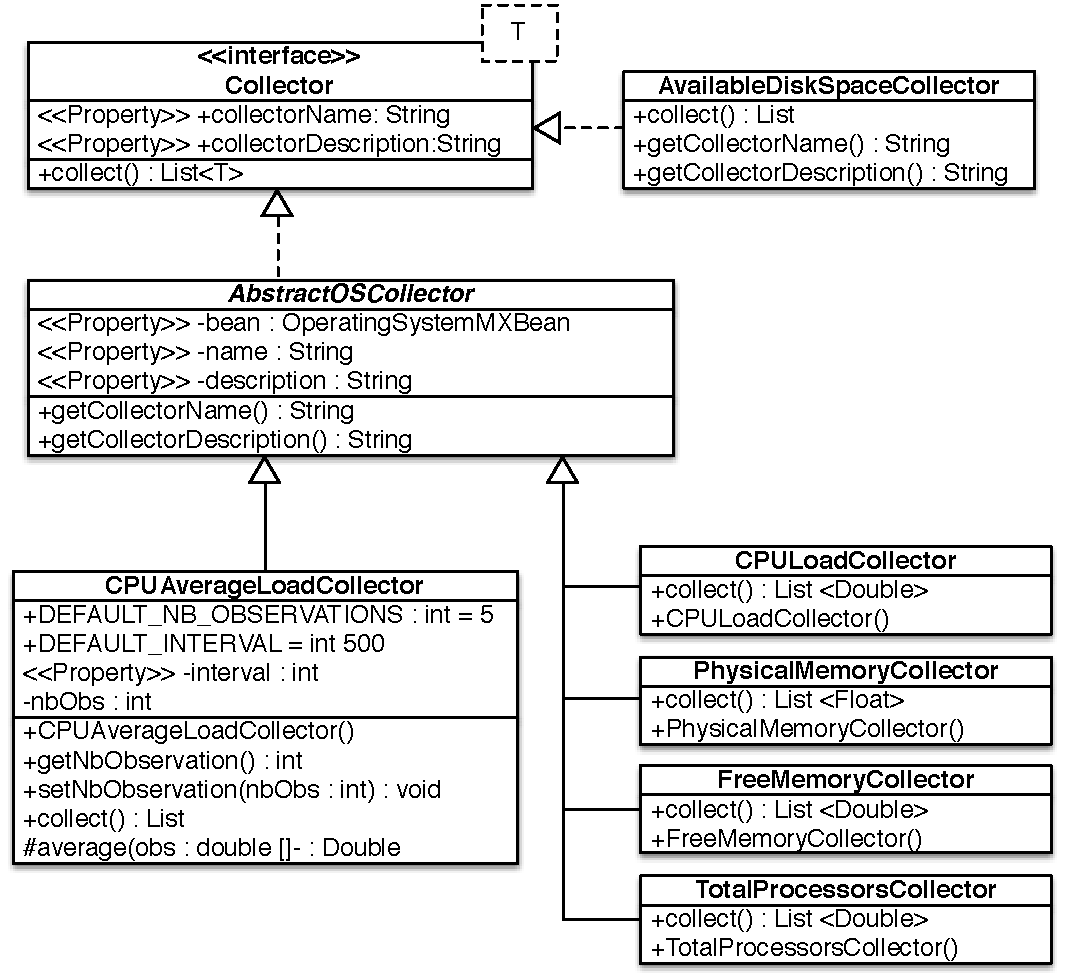
\includegraphics[width=15cm]{figuras/CollectorUML2.pdf}
   \caption{Diagrama de classes dos coletores de contexto}
   \label{fig:collectorUML}
\end{figure}

Cada instância de Node Manager possui um conjunto de coletores (um para memória e um para processadores), os quais realizam a coleta num intervalo pré-definido. Os coletores são executados por uma \textit{thread} independente e possuem um intervalo de 30 segundos entre as coletas para não causar sobrecarga ou interrupção no  processamento das tarefas \textit{MapReduce}.

%
%After the collector integration, changing the scheduling behavior was possible due to the now available information about the real resources of a given node. Further information about the results gotten from the collector integration and modified scheduling can be found at the chapter \ref{chap:Experiments and Results}.

%-------------------------------------------------------------------
\section{Comunicação Distribuída}
\label{sec:zookeeper}
Para que a informação coletada pelos coletores de contexto possa afetar o escalonamento é necessário que exista uma maneira para os Node Managers transmitirem os dados atualizados ao escalonador, a ferramenta escolhida para esta tarefa foi o ZooKeeper.

A flexibilidade oferecida através dos \textit{zNodes}, permite que qualquer estrutura de dado seja inserida como informação do \textit{zNode}. Optou-se por utilizar uma Tabela Hash, o que permite realizar a tarefa com apenas um \textit{zNode} e possibilita aos Node Managers a inserção das informações e ao escalonador o monitoramento de maneira simples.

Na solução adotada há apenas um Watcher, o escalonador, que monitora o \textit{zNode} da Tabela Hash. Qualquer alteração na tabela dispara uma \textit{callback} no escalonador, que por sua vez percorre a tabela a procura das modificações e realiza as alterações pertinentes nas informações sobre os recursos. Esta abordagem permite que o escalonador realize operações apenas quando necessário e não desperdice tempo acessando a tabela quando não houverem atualizações a fazer.

Na figura \ref{fig:zk} é possível visualizar a estrutura adotada no trabalho. Uma discussão possível de ser feita é sobre a decisão de utilizar somente 1 \textit{zNode} para toda tabela e o impacto disto em um cluster de 100 nós ou mais. Seria possível utilizar 1 \textit{zNode} para cada Node Manager, porém isto poderia fazer com que as \textit{callbacks} se acumulassem e o escalonador teria muitos processos apenas para atualizar os dados, uma vez que cada atualização geraria uma callback.

\begin{figure}[!hbtn]
   \centering
   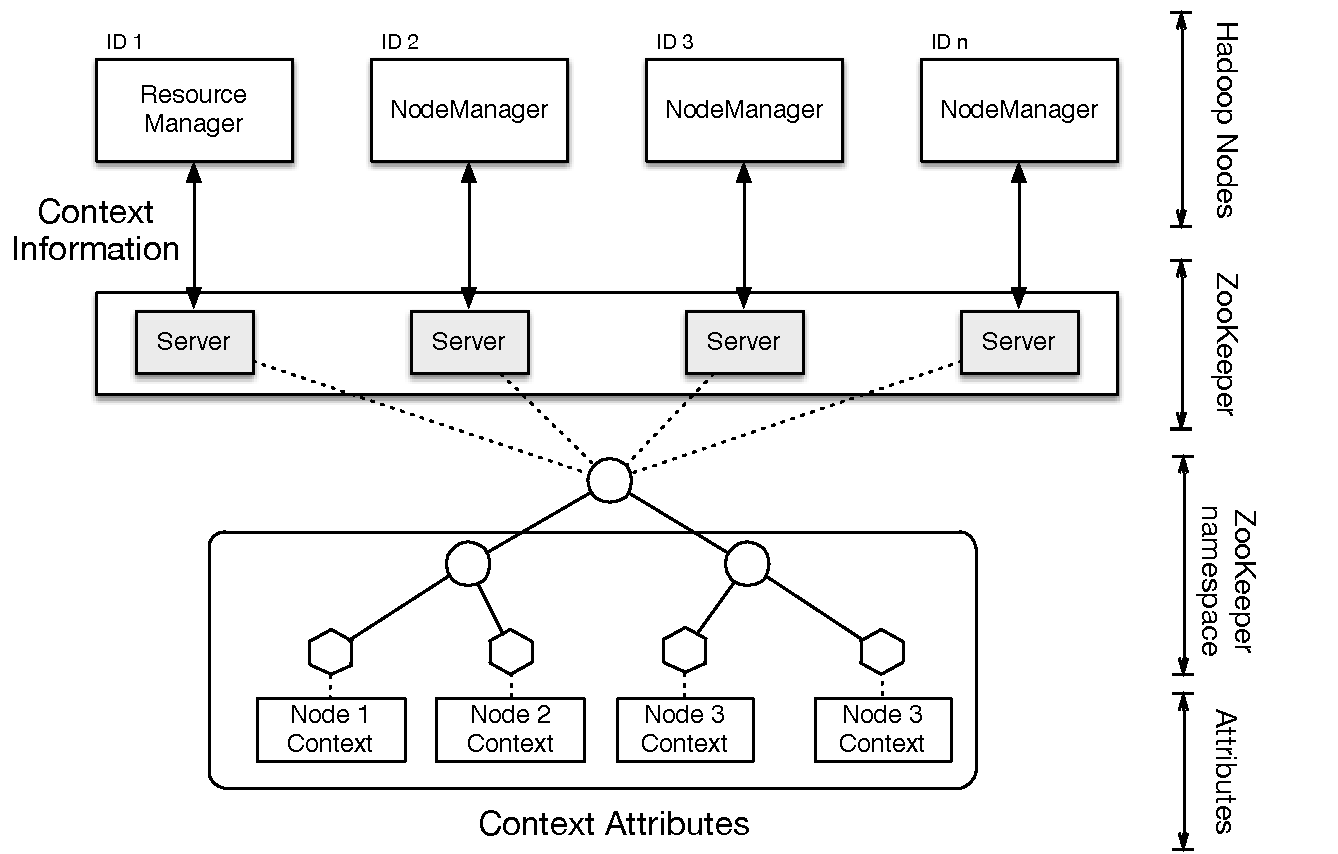
\includegraphics[width=15cm]{figuras/Zookeeper.pdf}
   \caption{Estrutura do ZooKeeper}
   \label{fig:zk}
\end{figure}

Como a solução escolhida apresenta dois papéis de clientes ZooKeeper, a seguir encontra-se uma explicação aprofundada de cada um destes papéis.

\begin{itemize}
	\item Cliente de Monitoramento: o papel de monitor é desempenhado pelo escalonador. O escalonador implementa a interface Watcher, fornecida pelo ZooKeeper, e monitora o \textit{zNode} que contém a Tabela Hash. No momento da inicialização o escalonador cria um \textit{zNode} e insere uma Tabela Hash vazia como informação, então finalmente, inicia o monitoramento do \textit{zNode}. Quando a \textit{callback} é acionada, a \textit{thread} percorre a tabela em busca de qual informação foi atualizada, atualiza os dados do escalonador e reinicia o monitoramento.
	
	\item Clientes de Atualização: o papel de atualização é realizado pelos Node Managers. Cada Node Manager lança, no momento de sua inicialização, uma \textit{thread} que faz a coleta de dados e caso haja alteração com relação à ultima leitura insere os dados atualizados na tabela hash. A coleta dos dados é realizada a cada 30 segundos, média de tempo observada em \textit{containers} executados em um \textit{cluster} de funcionamento normal.
	
\end{itemize}

%-------------------------------------------------------------------
\section{Solução Implementada}
\label{sec:solucao}

%TODO descrever geral,
%TODO colocar imagem da solução

\subsection{Integração dos Coletores de Contexto}
%TODO explicar como os coletores são inseridos na aplicação

\subsection{Integração dos Clientes}
%TODO explicar como os clientes zk interagem